% This is samplepaper.tex, a sample chapter demonstrating the
% LLNCS macro package for Springer Computer Science proceedings;
% Version 2.20 of 2017/10/04
%
\documentclass[runningheads]{llncs}
%
\usepackage{graphicx}
\makeatletter
\providecommand{\bigsqcap}{%
  \mathop{%
    \mathpalette\@updown\bigsqcup
  }%
}
\newcommand*{\@updown}[2]{%
  \rotatebox[origin=c]{180}{$\m@th#1#2$}%
}
\makeatother

\usepackage{color}
\usepackage{amsmath}
\usepackage{amssymb}
\usepackage{csquotes}
\usepackage{todonotes}
% Used for displaying a sample figure. If possible, figure files should
% be included in EPS format.
%
% If you use the hyperref package, please uncomment the following line
% to display URLs in blue roman font according to Springer's eBook style:
\usepackage{hyperref}
\renewcommand\UrlFont{\color{blue}\rmfamily}

\begin{document}
%
\title{Assuring Confidence in the Perception Chain of Highly Automated Vehicles
\thanks{Funded by the Deutsche Forschungsgemeinschaft under grant number 392437295.}}
%
%\titlerunning{Abbreviated paper title}
% If the paper title is too long for the running head, you can set
% an abbreviated paper title here
%
\author{Werner Damm\inst{1} \and
Martin Fr\"anzle \inst{1} \and
Willem Hagemann \inst{1} \and
Astrid Rakow \inst{1} \and
Mani Swaminathan \inst{1}}
%
\authorrunning{W. Damm et al.}
% First names are abbreviated in the running head.https://www.overleaf.com/1268442994rnstkwtzmypt
% If there are more than two authors, 'et al.' is used.
%
\institute{University of Oldenburg, Germany \\
\email{\{damm, fraenzle, hagemann, rakow, swaminathan\}@informatik.uni-oldenburg.de}\\
}
%
\maketitle              % typeset the header of the contribution
%
\begin{abstract}
%The abstract should briefly summarize the contents of the paper in 15--250 words.
%\keywords{First keyword  \and Second keyword \and Another keyword.}
We address one of the key challenges in \emph{assuring safety of autonomous} \emph{learning-enabled cyber physical systems}: how can we achieve confidence in the perception chain? We present a methodology and supportive architecture which allows to mathematically prove that the risk of misperceptions of \enquote{relevant} environmental artifacts of a highly autonomous vehicle (HAV) is less than a given level of societally accepted risk. The method requires the derivation of quality guarantees for sensors in different \enquote{Operational Design Domains (ODDs)}  as encouraged by the NHTSA \cite{NHTSF}, and proposes to dynamically adjust thresholds for accepting classification results for those individual artifacts of the environment whose misclassifications comes with drastic safety risks. 

\keywords{Learning-enabled cyber physical systems, Highly Automated Vehicles, Learning Algorithms, Safety Assurance, Perception Chain}
\end{abstract}
%
%
\section{Introduction}
\textcolor{red}{The \}

Assuring the safety of HAV entails assuring, that what the ego car beliefs to be true about its environment, and actual ground truth, rarely differ for all aspects which are relevant for ensuring the safety of the ego vehicle. How rare is rare enough is a matter of societal debates -- e.g. the German Department of Transportations requires HAVs to reduce the overall rate of fatalities. This paper answers the following question: if  r  is the level of societally accepted risks budgeted for misconceptions, how can we mathematically prove that perception of \enquote{relevant} environmental artefacts err at most with rate r? (We will clarify the vague term \enquote{relevant} in the text below)

We provide a mathematical setting for addressing this challenge, which is based on a reference architecture for the key functional ingredients of the perception chain. While clearly each OEM will have highly proprietary implementations, there seems to an emerging consensus in ongoing and currently prepared projects on Verification and Validation of HAVs in Germany, that an agreement on a functional reference architecture is both desirable and achievable. Our proposal for the reference architecture uses labelled occupancy grids for fusion of data from radar, lidar, video, etc, and as interface to learning-algorithms based components for classifying objects in the environment of the ego-vehicle according to a (to be standardized) partially ordered ontology. We assume that each artefact in this ontology comes with class definitions characterizing both static and – if applicable – dynamic aspects, such as e.g. ODD dependent models for typical traffic behavior (e.g. characterizing variations in lateral and longitudinal acceleration of vehicles in a neighboring highway lane, or of pedestrians in an urban pedestrian crossing), and will exploit such knowledge to reduce misclassification rates. The reference architecture also requires for each sensor the capability to identify harsh environment conditions (where no sufficiently tight bounds for risk of misconceptions can be given), and exploits this information in mechanisms for sensor fusion. The reference architecture also gives formal meaning to the vague term \enquote{relevant} environmental artefact, in that the maneuver component provides feedback to the criticality of achieving high confidence information for individual fields in the occupancy grid: errors in misclassifications of objects only count, if they relate to such critical classifications. Finally, we propose a safety net reducing likelihood of misclassifications, in declaring \enquote{blindness} for classifications, where neither the evidence for existence of an artefact a nor the evidence for absence of a is sufficiently strong – such declaration of \enquote{blindness}, if sustained over several cycles for relevant artefacts, will automatically induce minimal risk maneuvers (as does any detected usage of the HAV outside the allowed ODD).

The main result of this paper is a methodology for formally establishing bounds on the risks of misperception for artefacts labelled \enquote{critical} by the maneuver layer. This proof is composed bottom up by propagating quality guarantees along the different levels of the perception chain. We document this proof through justifications, giving for each level the reasons why the risk of misconception can be bounded. Such justifications could provide a tool for post-mortem accident analysis.

This paper is organized as follows: 
Section \ref{sec:mathmodel} defines a mathematical model of (ground truth) traffic flow in a given ODD, where observables are defined through the ontology and their associated classes. It then formalizes for a given ego car the partial knowledge the ego car acquires about its environment based on its perception chain, and refer to these as the ego car's beliefs about its environment. We then formally define the overarching safety requirement for HAVs in a given ODD, in relating the level of precision and risks of misconception between ground truth and beliefs of the ego vehicle. Section \ref{sec:refarchitecture} defines the reference architecture of the perception chain as outlined above.
Section \ref{sec:example} illustrates our proof methodology with a simple example. Section \ref{sec:proofrule} contains the formal proof rule and key elements of the underlying statistical arguments for bounding the level of risk. Section \ref{sec:relatedwork} discusses related work. We wrap up with a way forward in using this methodology.



\section{State of Art}\label{sec:relatedwork}
Highly automated vehicles are typically \emph{learning-enabled cyber physical systems} operating in an uncertain environment, where the learning about the \emph{dynamic} environment is enabled through \emph{inaccurate} sensors. This renders an exact inference of the state of the environment infeasible, necessitating representations of the \emph{uncertainty} in inferring about a dynamic environment through inaccurate sensors. Such representations of uncertainty have been investigated a.o. within the paradigm of \emph{probabilistic robotics}~\cite{probrob}, particularly as applied to vehicle localization in urban environments~\cite{Thrun2007,Thrun2009,Thrun2010}. In these and related works such as~\cite{Perrolaz2014, moras2014}, the environment uncertainty is represented as \emph{probabilistic
beliefs}. 


As an example, consider a popular perception technique like simultaneous localization and
mapping [5] (SLAM), which is used for determining the current position of an autonomous
vehicle. The estimated position of the vehicle and the coordinates of other entities in the map
are often assumed to have Gaussian noise. Aside from localization and mapping, another critical
perception challenge for autonomous vehicles is obstacle detection and tracking [8,27].
Camera and laser range finders are used to locally detect and avoid obstacles during navigation
for a previously constructed map. This is particularly useful in the presence of dynamic
objects whose locations are not fixed in the environment map. The uncertainty in the parametric
models representing the obstacles is usually also modelled using Gaussian random
variables





\section{Mathematical Model}\label{sec:mathmodel}
We assume as given a partially ordered ontology (cf. Section~\ref{sec:proofrule} for the formal definition) containing all relevant environmental artifacts for HAV. Initiatives towards identification of such an ontology are currently part of a number of R\&D projects on HAV, including the PEGASUS project\footnote{\url{www.pegasusproject.de}}. The ordering relation reflects the degree of precision of classification of objects, with $\bot$ (read: bottom) representing inconsistency, and $\top$ (read: top) denoting \modify{zero}{no} knowledge. The ontology contains different kinds of artifacts, e.g. relating to weather conditions (\del{fog, }rain, snow, \ldots), road configurations (x-lane highway, T-type \del{x lane} intersection, \ldots), road conditions (dry, icy, \del{aquaplaning} \ldots), roadside infrastructure (traffic signs, traffic lights, \ldots), traffic participants (car, truck, \del{bicycle, }pedestrians,  animals, \del{obstacles,} \ldots), and surroundings \del{of road segments} (trees, buildings, \ldots). Objects in different categories are \modify{related by relations,}{in relations} and form separate sublattices, which are turned into a complete lattice by \modify{introducing}{adding} a new top element. \modify{In this paper}{Here} we \del{will} only refer to weather conditions, traffic-situations and\del{traffic} -participants. Such ontologies are today in regular use as semantic basis for driving simulators such as SiLab\footnote{\url{wivw.de/en/silab}}. \del{Sample ordering relations in the category of traffic participants are shown in Fig. \ref{fig1} below.
\begin{figure}
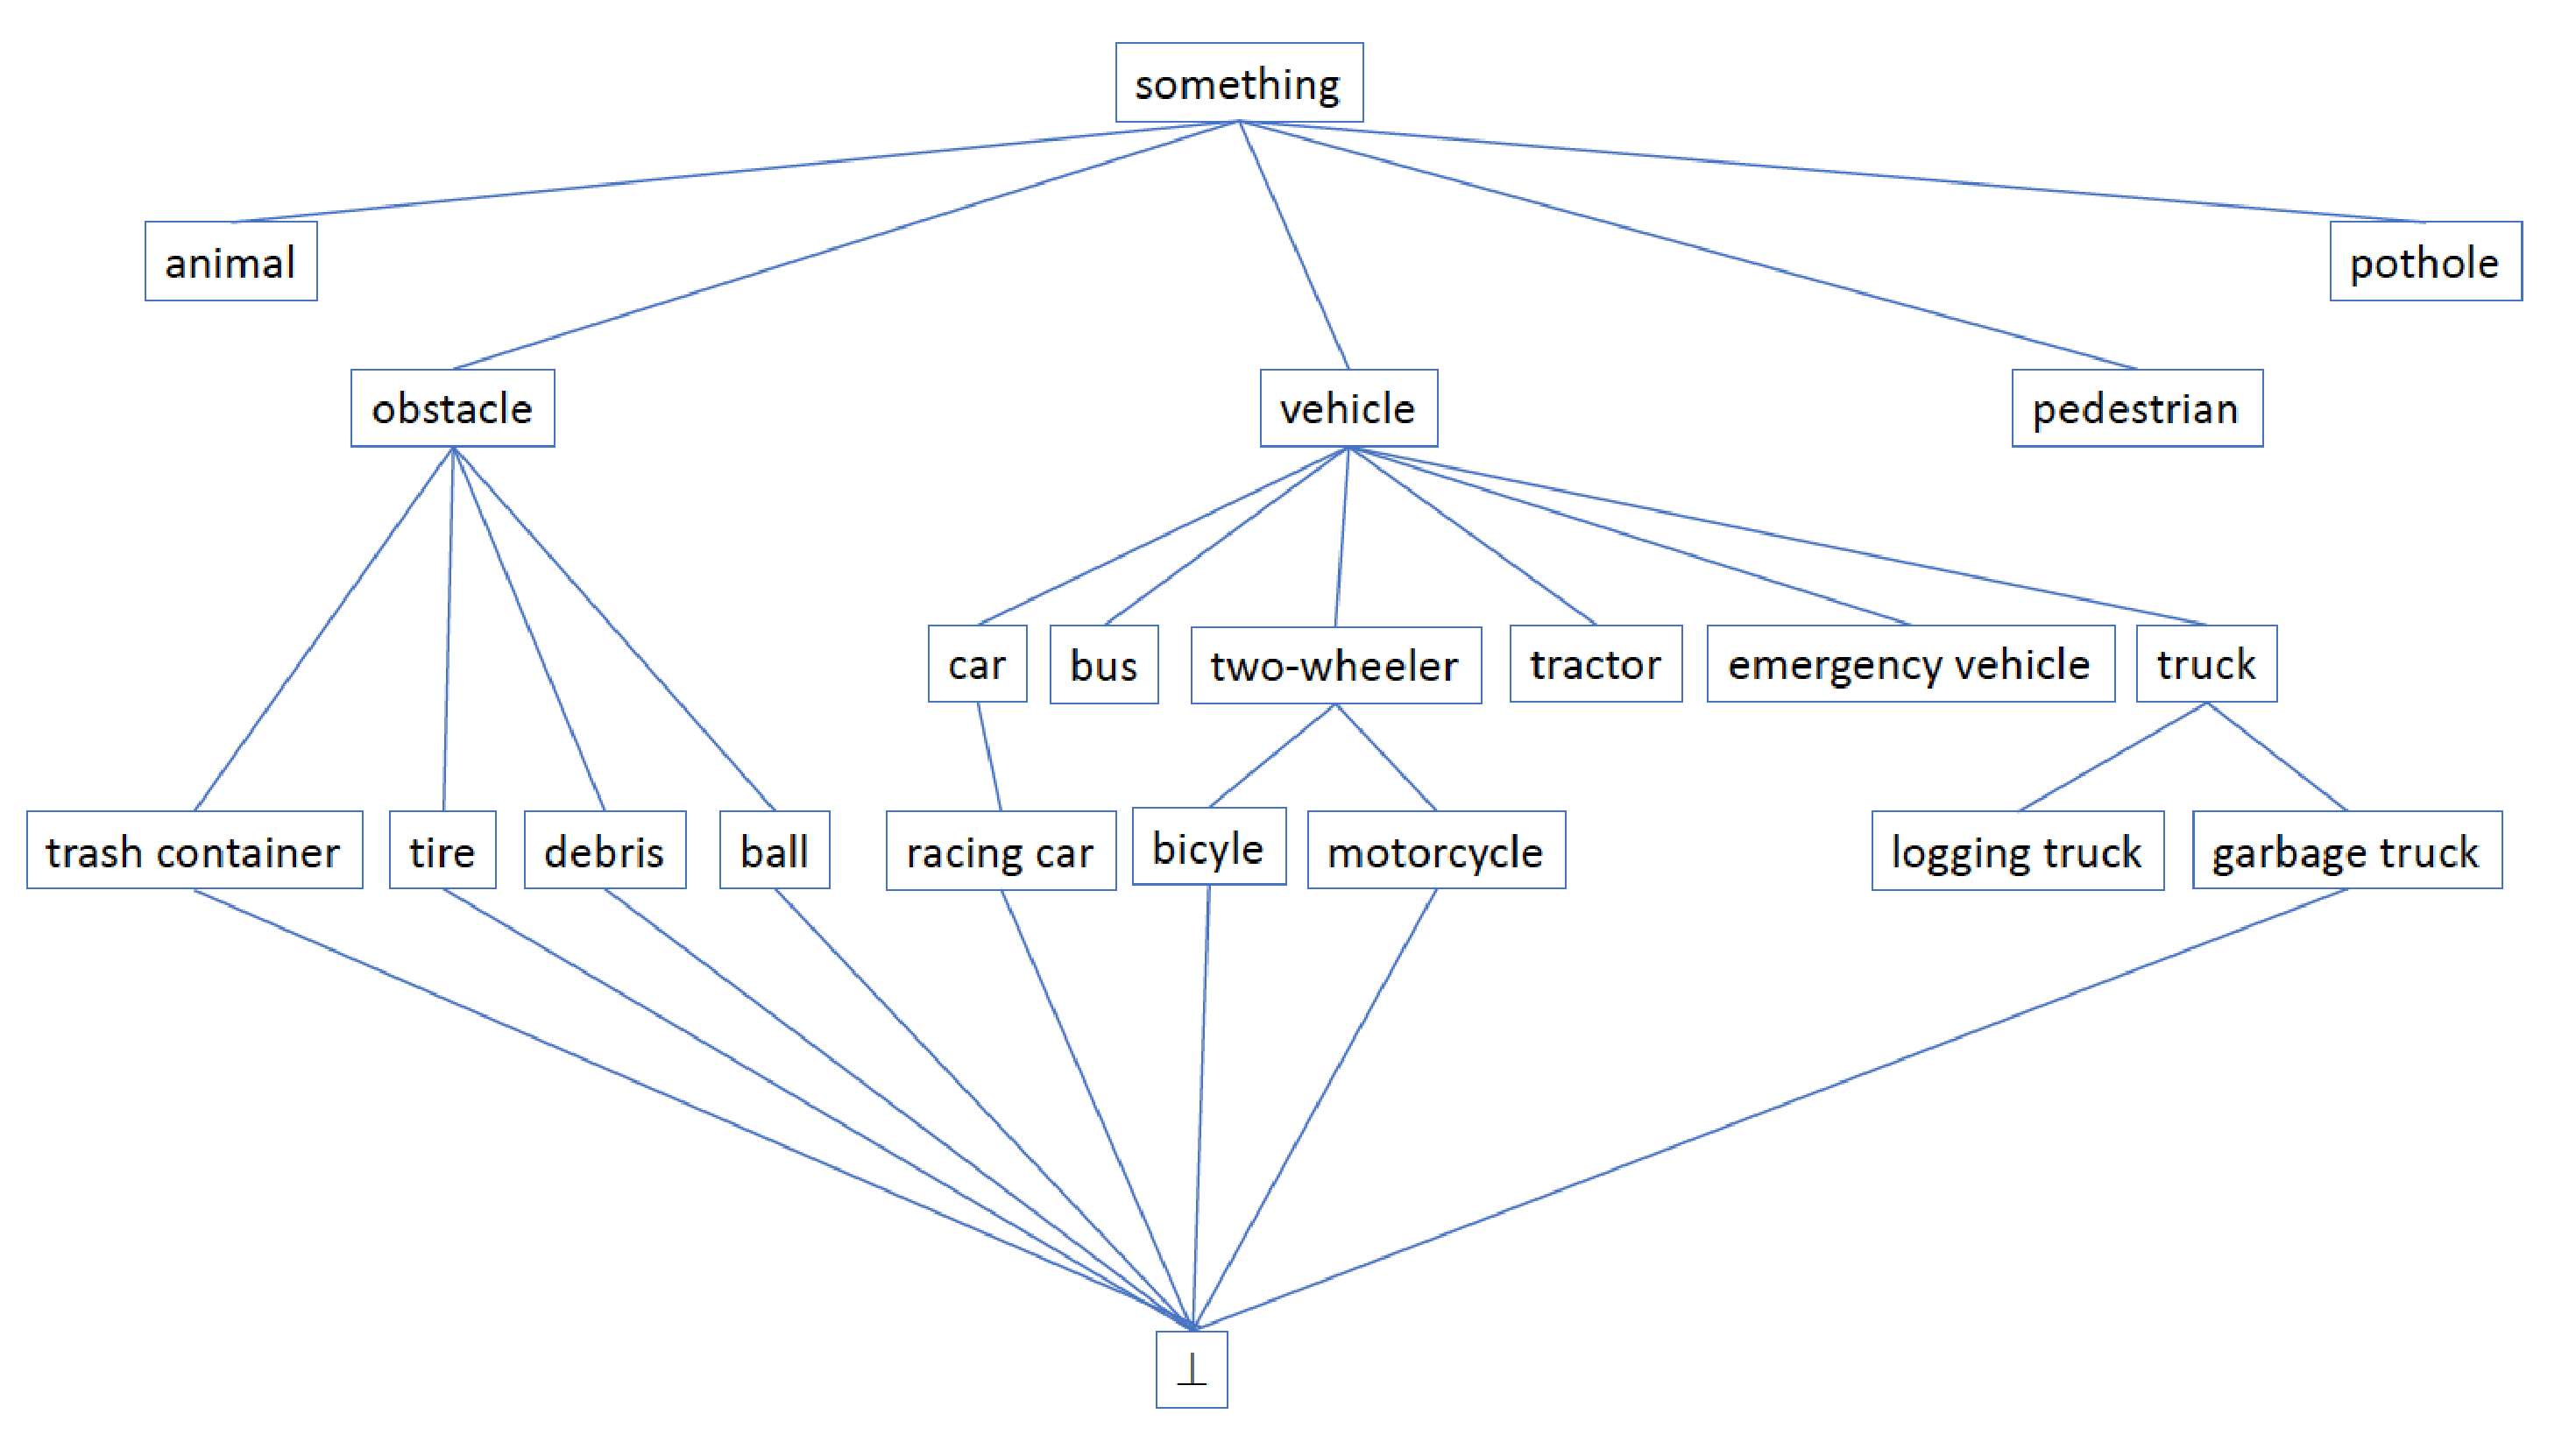
\includegraphics[width=\textwidth]{fig1.eps}
\caption{Sample ordering relations in the category of traffic participants} \label{fig1}
\end{figure}}

With each artifact  \emph{a}  in the ontology, we assume as given a specification of its HAV-related aspects through a class definition $c_l(a)$. For artifacts of type road configurations, this includes specification of all geometric aspects including slope, number of lanes, width of lanes, etc. Road configurations are built from segments of a parametric length. An operational design domain ODD is defined by constraints on types of road configurations, and constraints on prevailing weather conditions and road conditions. For each artifact \emph{veh} of type vehicle, attributes of $c_l(veh)$ include the type of an instance of class road configuration, on which the vehicle is currently located, as well as its position\del{ such as its longitudinal and lateral position on some lane of this instance of class road configuration}. Moreover, each vehicle maintains its beliefs about its environment in appropriately typed attributes. \modify{Figure \ref{fig2} below depicts the beliefs of ego driving on a country road: it believes }{For example a car, ego, driving on a country road may believe} the road surface is dry, that there is an obstacle in 250 m distance ahead blocking the lane, and that some vehicle of unknown type is approaching on the opposite lane. Importantly, $c_l(veh)$ contains as well a characterization of ODD-dependent dynamics of \emph{veh}. We assume that these are given by probabilistic hybrid automata (PHA) \cite{pha}, where mode changes are triggered based on believed changes of road configurations, weather conditions, road conditions, and observations of surrounding traffic and roadside infrastructure. A key point to be exploited is, that behavioral models are increasingly unconstrained along the generalization hierarchy: e.g., for class vehicle, the associated probabilistic hybrid automaton is constructed from those of the next level of specialization by introducing a new start state, branching non-deterministically into the entry states of the PHA of cars, two-wheelers, trucks, emergency vehicles, etc. Similarly, we assume such models for pedestrians, animals, obstacles etc.\del{
\begin{figure}
    \centering
    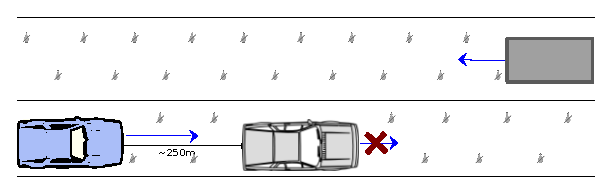
\includegraphics[width=0.45\textwidth]{obstacle+vehicle2.eps}
    \caption{Beliefs of ego}
    \label{fig2}\label{fig:obstacle}
\end{figure}
}
Based on this, we can define a mathematical model of traffic evolution from the perspective of a given ego-vehicle. We define the electronic horizon of the ego vehicle to be the best-case range of perception of its on-board sensory system, and for simplicity of exposition \del{in this paper }assume this to be given by a rectangle aligned to the current pose of the ego vehicle centered at the geometric center of the ego vehicle. \del{We call back- resp.\  front-horizon of ego the uttermost road segment still visible behind resp.\ in front of the car through its electronic horizon. }The mathematical model is an infinite state transition system, whose state space is constructed as follows:
\modify{\begin{itemize}
\item It contains for each point in time \emph{t}  all instances of road segments extending from the instance on which the ego car is currently positioned completely covering its electronic horizon;
\item For each of the above road segments, it contains for time \emph{t} the position and speed of all vehicles on the road segment, as well as road and weather conditions, positions of pedestrians, animals, obstacles, etc.
\end{itemize}}{
It contains for each point in time \emph{t}  all instances of road segments extending from the instance on which the ego car is currently positioned completely covering its electronic horizon; For each of the above road segments, it contains for time \emph{t} position and speed of all vehicles on the road segment, as well as road and weather conditions, positions of pedestrians, animals, obstacles, etc.}
The (dense time) transition relation of the mathematical model 
\modify{is constructed as follows:
\begin{itemize}
\item New road segments are generated at the front- and lateral horizons by randomly instantiating new instance of class road segments while obeying the constraints of the ODD.
\item These new road segments are randomly attributed with road conditions and weather conditions observing consistency constraints and physical laws, and randomly filled with vehicles of randomly chosen type, with speeds and relative distances compliant to real observed traffic flow under the given ODD, as captured by the associated PHA.
\item Where applicable, pedestrians are positioned randomly on newly generated road segments, observing traffic rules and dynamic models of pedestrians.
\item Evolution of instances of objects of classes vehicles, pedestrian, animals follow the associated dynamic models.
\item The evolution of the ego-vehicle follows the driving strategy determined from its beliefs about its environment as given by a probabilistic hybrid automaton.
\end{itemize}}{is determined by following a driving strategy based on ego's beliefs where the environmental constraints are instantiated randomly according to the ODD and  the dynamic models associated with other traffic participants are considered.}
We refrain for space reasons from giving the formal definitions, and refer to this transition system by \textit{TS(ego)}. A state of \textit{TS(ego)} is given by a valuation of all its observables. A run of \textit{TS(ego)} defines for each observable its evolution over time, thus including trajectories of all vehicles, pedestrians, animals, obstacles within ego's electronic horizon, including the evolution of the beliefs of the ego vehicle, and the evolution of its perceived road segments. We call $RUNS(TS(ego))$ the set of all runs of \textit{TS(ego)}.

We can now formalize the meta requirement for the quality of the perception chain, up to the (to be defined) defined notion of relevance, in a probabilistic linear time temporal logic, with observables defined by valuations of all attributes of all instances of classes within the electronic horizon of ego, over a typed first-order signature induced by the types of attributes in the ontology. Ideally, for each point in time, the ground truth of all relevant artifacts in ego's electronic horizon, in particular position and speed of surrounding traffic participants, road- and weather conditions, coincide exactly with ego's beliefs about these artifacts. We must relax this unachievable ideal by considering standard measurement errors, and allowing classifications to be vague, as long as they are correct with respect to the ordering relation in the ontology, i.e.\ the ground truth classification is a specialization of the believed classification. While misclassifications and misperceptions will occur, we want these to be bounded by the societally accepted level of risk. Assuming for each artifact $a$ a metric $d_a$ to measure the distance between ground truth and beliefs of $a$, and a safe level of measure tolerance $\delta_a$. We want almost always these to be consistent for a minimal time period $\Delta$ sufficient to take safe maneuver decisions for the HAV. This leads to the following formal requirement on the confidence of the perception chain of the HAV vehicle ego:
\begin{align}\label{eq:safeperception}
	\textit{Safe}\_ &\textit{perception}(ego) =\forall a \in \textit{observables}(\textit{TS(ego)}):  \Box (\textit{relevant}(a) \Rightarrow\\ 
			&P(\neg(\Box_{\leq\Delta}d_a(a, \textit{belief}(a)))\leq \delta_a) < r).\nonumber
\end{align}

We note that the precise definition of this metric must deal both with misclassifications and errors in measurement. The actual setting in the paper will resolve this by addressing measurement errors and misclassification errors separately, following the reference architecture of the perception chain. 

\section{The functional reference architecture of the perception chain}\label{sec:refarchitecture}
This section develops a functional reference architecture for the perception chain allowing to provably bound the risk for misperceptions. The following principles guided this proposal:
\begin{enumerate}
\item It must be possible to bound the contributions to risks for each component of the perception chain.
\item This entails the need to specify for each element in the perception conditions under which this element can be \enquote{trusted}. Violations of such conditions must be monitored and -- if persistent -- must induce declaration of \enquote{blindness}, automatically inducing minimal risk maneuvers.
\item The reference architecture must provide guidance as to the degree of precision of perception required for current maneuver decisions
\item The reference architecture must support trade-off between maximal availability and maximal safety.
\end{enumerate}
We discuss the implications of these design principles in separate subsections, along the flow through the perception chain.

\subsection{Quality criteria for sensor components}\label{subsec:quality}

While radar systems are widely deployed for variants of ACC systems and emergency breaking systems, their integration in level 3, 4, or 5 HAVs constitutes a completely different operational context, because the overall safety case can no longer rely on human supervision of the environment of the ego car. Well known phenomena such as ghost objects stemming from undesired and uncontrollable reflections, or \enquote{stealth type cars} such as the VW beetle, or simply reflections induced by metal-coating of truck planes are but examples of a plethora of phenomena, which all influence quality of object detection through radar. With the transition to level 3, 4, 5 systems, quality criteria must take a more rigid form: we must be able to quantify the risks of missing objects, or showing ghost objects. Similar types of distortion of perception are well known and documented for Lidar systems in certain types of rain conditions, for video systems in certain types of lighting conditions, etc. We propose a uniform quality measure for different type of sensor systems, by assessing their capability to contribute to detecting all relevant objects in the what is often called the occupancy grid enclosing the ego car. Specifically, we take a suitable 3d extension of the electronic horizon of the ego vehicle, and assume a sufficiently fine grained, not necessarily homogeneous partitioning of this 3d space, and refer to this as \emph{occupancy grid(ego)}. We view sensors as labelling partitions of the occupancy grid, providing information about whether a given sensor has identified some artifact in this grid partition, depending on sensor type filled with additional information such as speed (for radar), temperature (for infrared), gray-scale distribution of pixels for video cameras, \ldots, typically as distributions with confidence levels, e.g. regarding the likelihood of some artifact being located in this grid partition. 

We provide a formal quality requirement on sensors by adapting the safe perception requirement in formula (1). Specifically, for a given position \textit{pos}  of sensor  \textit{s}  on vehicle ego, let us denote by \textit{visible(s,pos)} the coherent subspace of the occupancy grid covered by sensor \textit{s} when mounted at this position, then for any relevant artifact  $a$, and any property  \textit{label($a$)} discernable by  \textit{s}  in this position, we would want the sensor \textit{s} to almost always, up to some bounded risk $r_s$, correctly label the grid field with \textit{label($a$)} at time $t$, when $a$ is at a visible grid partition in ground truth, as determined by the state of \textit{TS(ego)} at that point in time:

\begin{align}\label{eq:safelabelling(s,pos)}
    \textit{Safe}\_&\textit{labelling(s,pos)} \equiv 					\\		
 & \forall a\in\textit{ observables(TS(ego))}\forall p \in \textit{occupancy grid(ego)}:\nonumber\\  
& \Box (\textit{relevant}(a) \land a \textit{ is at } p\land p\in \textit{visible(s,pos)} \nonumber\\
& \Rightarrow P(\neg( \Box_{\leq\Delta} d_{a,s}(a,\textit{label}(a))\leq\delta_{a,s}))) < r_s\nonumber
\end{align}

In this formula, we interpret the predicate \textit{visible(s,pos)} \emph{dynamically}, providing for subspaces of the occcupancy grid to be temporarily blocked through artifacts such as other vehicles, or buildings, etc. Moreover, since phenomena such as glare, fog, heavy rain etc will have strong negative impact on achieving sufficiently precise distances between beliefs and ground truth, we propose to characterize for each sensor what we call \emph{adverse} conditions. Only by using self-correcting sensors such as radar systems identifying ghost objects and separating out such adverse conditions can we obtain a sufficiently tight bound on the risks of incorrect labelling of the occupancy grid, to achieve an overall risk tolerated by society. The down side is the need to then also identify reliably such adverse conditions; in this paper, we integrate such adverse conditions in our ontology, and then use the full power of the perception chain to learn sufficiently reliable classifications of adverse conditions, see next subsection. As in \cite{galbas}, we propose to use learning techniques from field observations to characterize adverse conditions for each sensor \textit{s} and to derive such quality guarantees. We now weaken formula (2) by weakening the criteria for sufficient precision of beliefs in that no promises regarding precision are made when adverse conditions $ad$ occur:

\begin{align}\label{eq:safelabelling(s,pos,ad)}
\textit{Safe}\_&\textit{labelling(s,pos,ad)} \equiv\\  			
&\forall a\in \textit{observables(TS(ego))}\forall p\in\textit{occupancy grid(ego)}\nonumber:\\
&\Box(\textit{relevant(a)} \land a\textit{ is at p }\land p\in\textit{visible(s,pos)} \Rightarrow\nonumber\\
&P(\neg(\Box_{\leq\Delta} (d_{a,s}(a, \textit{label(a)})\leq \delta_{a,s}))\textit{ unless } ad)) < r_s\nonumber
\end{align}

Note that we can in particular encode the constraints of a given ODD in such adverse conditions, which thus entails that information of a sensor is not trusted if working outside the constraints of the ODD. OEMs compensate weaknesses of types of sensor systems by providing redundancy and diversity and using sensor fusion. To this end, let us define the class of labels stemming from different types of sensors. Let us assume for simplicity that the resolution of the grid corresponds to the  
\todo[inline,color={blue!100!white!33}]{\footnotesize AR: Ich finde die ad(s)/ Kontrakte sollten 3 Bereiche unterscheiden (1) vis(s1)und!vis(s2), (2) vis(s1)und vis(s2) und (3)vis(s2)und!vis(s1). Die Wahrscheinlichkeit von Falschaussagen sinkt in (2), aber die Qualitaet von (1) sinkt nicht wenn (2) weniger zuverlässig ist.}
We can derive a composed sensor s from fusing two qualified positioned sensors $<$s1,pos1$>$  and $<$s2,pos2$>$ to system s as follows:
%
\begin{itemize}
\item ad(s) is the disjunction of ad(s1) and ad(s2)
\item visible(s) = visible($<$s1,pos1$>$) $\cup$ visible($<$s2,pos2$>$)
\item for each $p\in $\textit{occupancy grid(ego)}:  \\
if p $\in$ visible($<$s1,pos1$>$) $\cap$ visible($<$s2,pos2$>$) then
\begin{itemize}
\item if $\neg$ad(s1)$\land\neg$ ad(s2) then\\
if label(s1)(p) $\land$ label(s2)(p) $\not=$ false 
\begin{itemize}
\item[] then label(s)(p) := label(s1)(p) $\land $label(s2)(p)
\item[] else label(s)(p) := $\bot$
\end{itemize}\todo{Weiss nicht wie man es besser machen soll, aber die Nichtmonotonie, dass man hier im besser informierten Fall pessimistischere Label zuordnet als wenn ein Sensor erblindet ist, stoesst mir auf.}
\todo[inline]{WH: das letzte if--then--else l\"asst sich zu "label(s)(p) := label(s1)(p) $\land$ label(s2)(p)" zusammenfassen (da $\bot$ ja gerade false repr\"asentiert).}
\item[] else if ad(s1)$\land\neg$ad(s2) then label(s)(p) := label(\textcolor{red}{s2})\todo[color={blue!100!white!33}]{AR: Ich hab hier s1 und s2 getauscht.}
\item[] else if $\neg$ad(s1)$\land$ad(s2) then label(s)(p) := label(\textcolor{red}{s1})
\item[] else if ad(s1) $\land$ ad(s2) then label(s) := $\bot$
\end{itemize}
\item[] else if p$\in$visible($<$s1,pos1$>$) $\setminus$ visible($<$s2,pos2$>$) then\\	
if $\neg$ad(s1)
\begin{itemize}
    \item[] then label(s) := label(s1)
	\item[] else if ad(s1) then label(s) := $\bot$
	\end{itemize}
	else if p $\in$ visible($<$s2,pos2$>$) $\setminus$ visible($<$s1,pos1$>$) then
	\begin{itemize}
	\item[] if $\neg$ad(s2) 
	\begin{itemize}
	    \item[]then label(s) := label(s2)
	\item[] else if ad(s2) then label(s) := $\bot$
    \end{itemize}
    \end{itemize}
\end{itemize}
Note that any detected inconsistencies are marked $\bot$. Also the combined sensor labels fields p with $\bot$ if p is only visible for one sensor, but this sensor cannot be trusted because of prevailing adverse conditions. We derive quality guarantees for sensor fusion in Section \ref{sec:proofrule}. For observations where both sensors are in non-adverse conditions, and both sensors observe p, then the risk of misclassifications is reduced to $r_{s1} \times r_{s2}$ if we can prove that misperceptions are stochastically independent under operating conditions favorable for both sensors, otherwise the risks for misperception of the fused systems for fields p visible to both sensors is min($r_{s1}$,$r_{s2}$).

Level 4 and 5 HAVs must guarantee by construction sensor completeness with maximal risk r: for all points in time, and all relevant fields p of the occupancy grid, there must at least be one positioned sensor operating in non-adverse conditions, such that p is visible for this sensor, and the risk of misperception by this sensor is smaller than r, unless there are multiple positioned sensors all operating in non-adverse conditions, which are stochastically independent under such conditions; in this case the products of their risk levels must be smaller than r. Since this property is more easily expressed using the formula derived in Section \ref{sec:proofrule} for sensor fusion, we formalize this key requirement of sensor completeness in Section \ref{sec:proofrule}.

\subsection{The functional reference architecture}

\begin{figure}
    \centering
    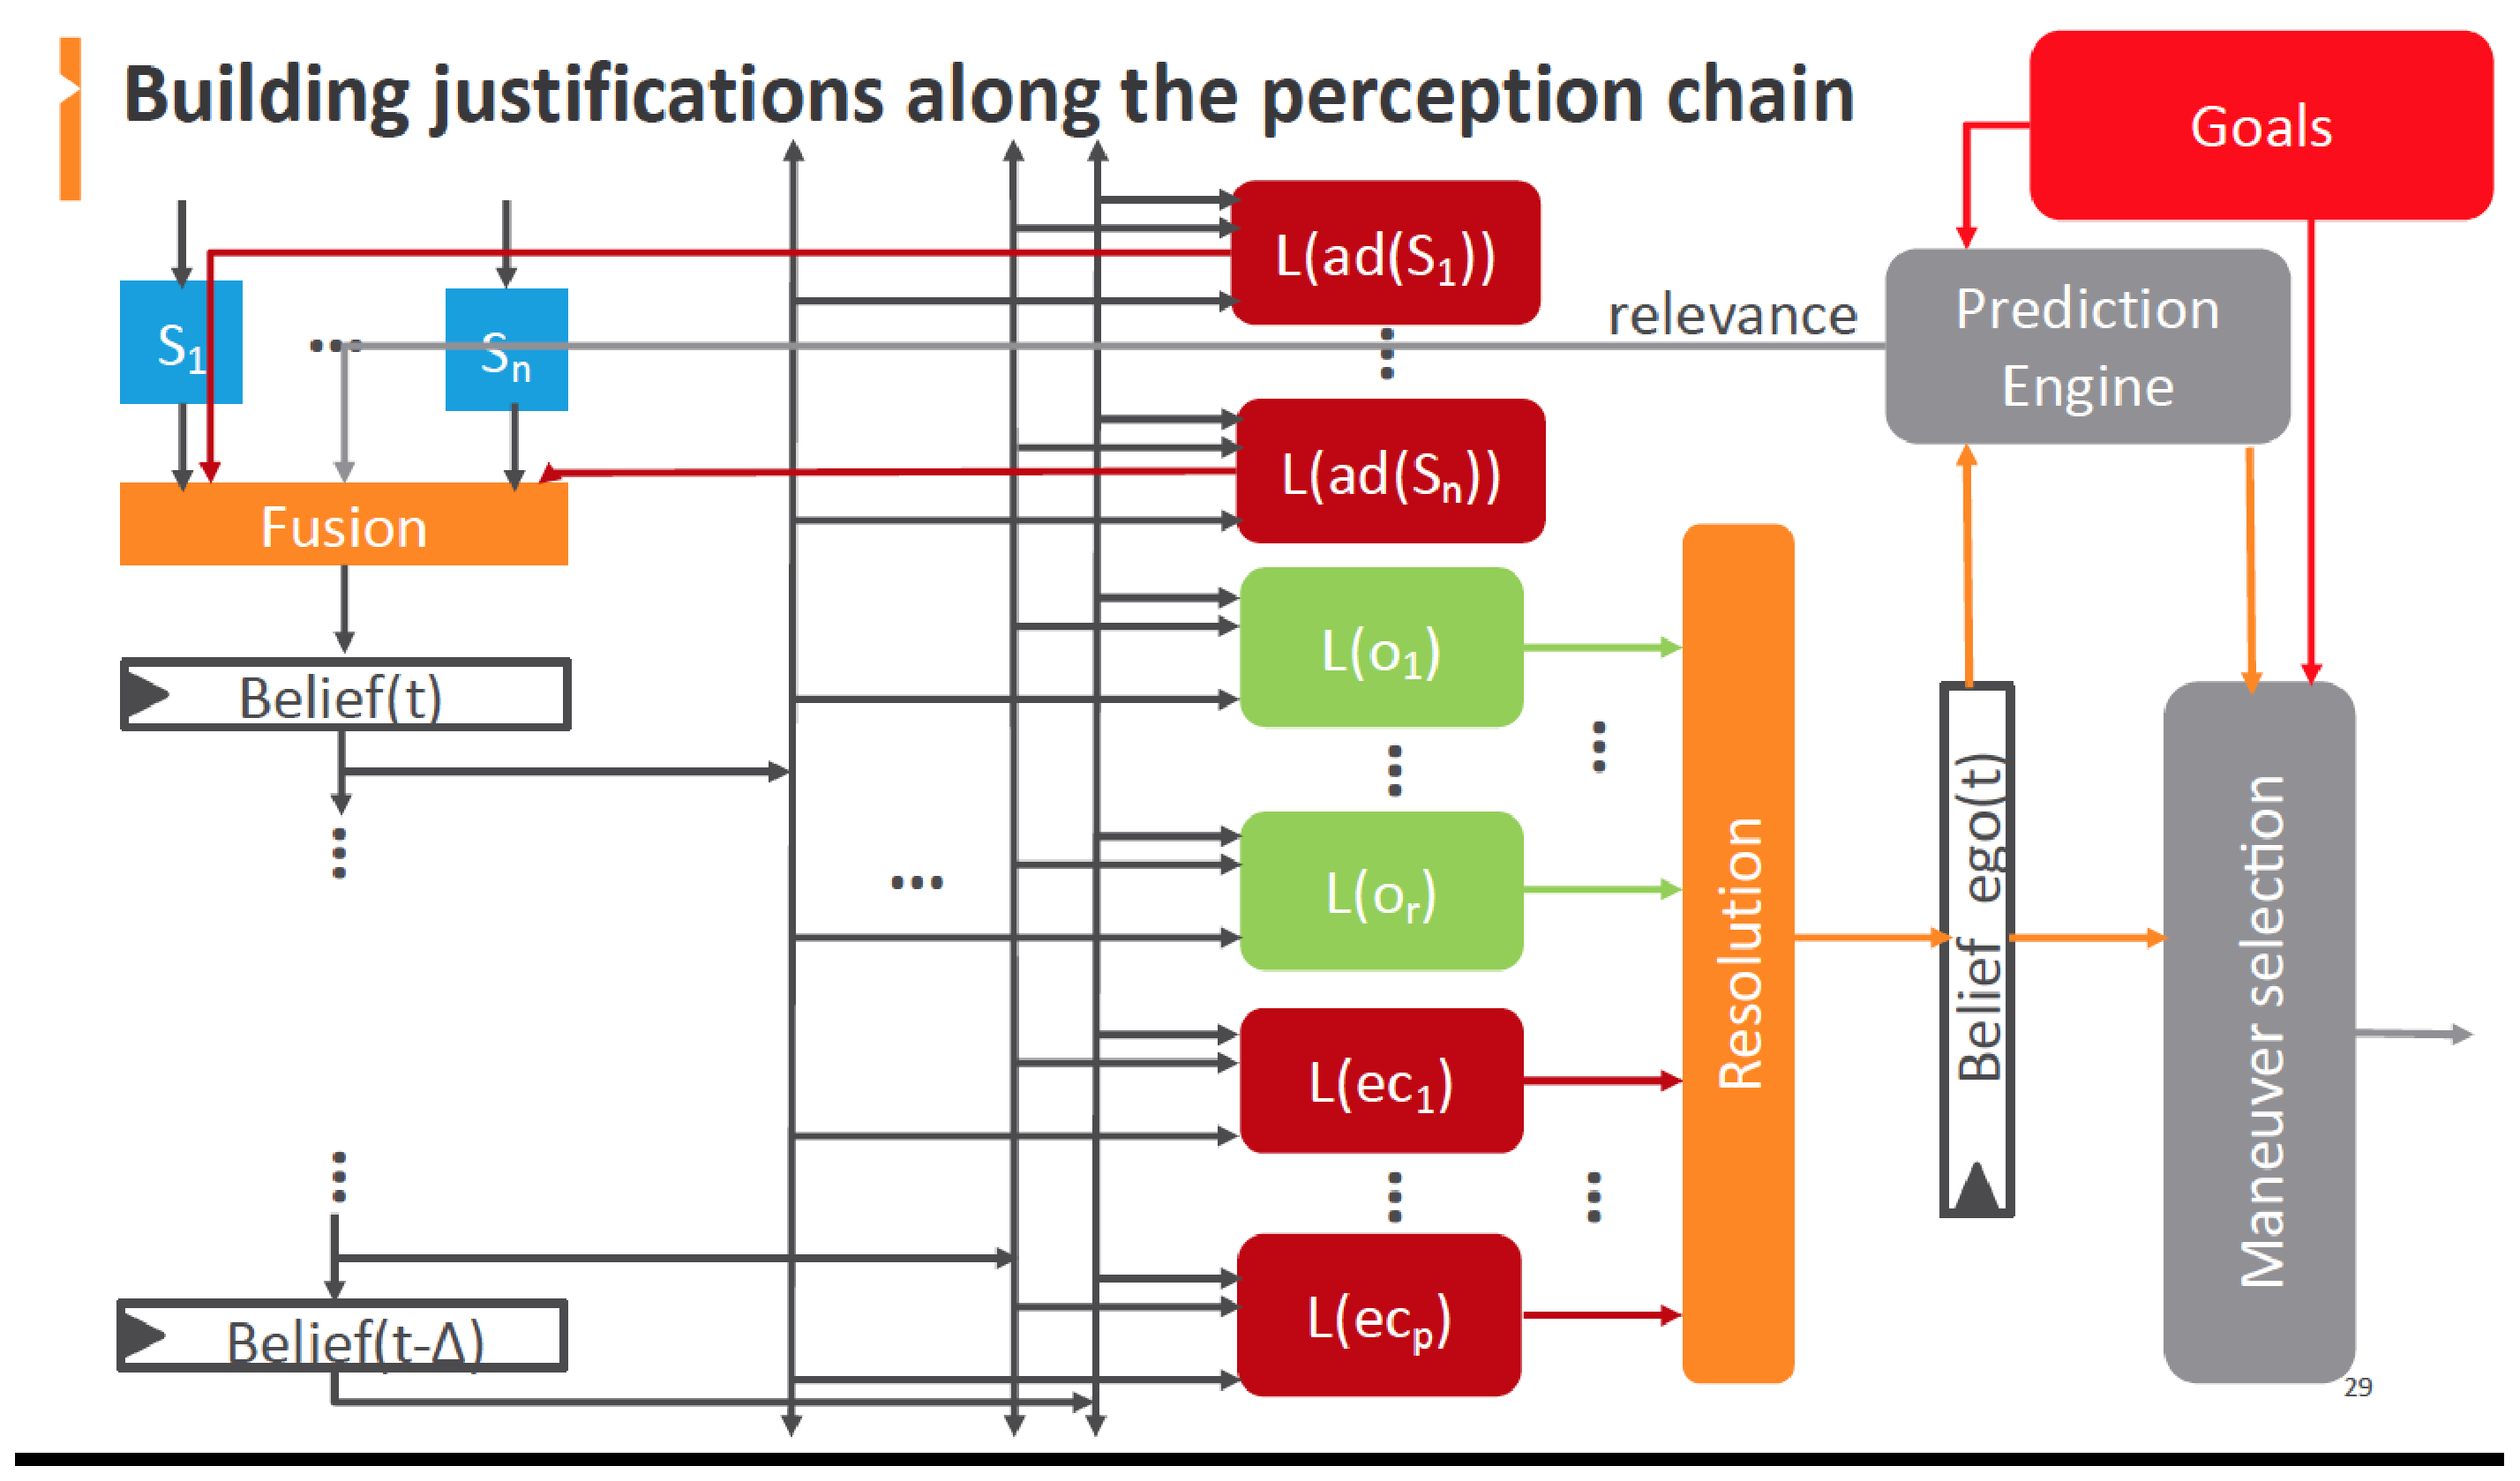
\includegraphics[width=\textwidth]{fig2.eps}
    \caption{Reference architecture}
    \label{fig:architecture}
\end{figure}
Figure \ref{fig:architecture} shows the proposed functional reference architecture of the perception chain, where belief(t) represents the labelled occupancy grid resulting from fusion of sensors s1 to sn, as discussed in Sect. \ref{subsec:quality}. We distinguish these from the complete reconstruction of the environment of the ego car, belief(ego), and assume that for each artifact  a in the ontology we have a dedicated learning component  L(a) for detecting both presence and absence of a in fields of the occupancy grid, see below. Note, that we assume that the prediction engine provides feedback about the relevance of fields in the occupancy grid, based on knowledge about the current beliefs of the ego car, and its current goals. Note also, that the learning components for identifying adverse sensor conditions are fed backwards into the sensor fusion unit. We propose the following measures to reduce the error of misperception:
\begin{enumerate}
\item To be able to exploit physical laws to optimize the prediction rate, we propose to maintain copies of such beliefs over some time window $\Delta$, and feed this into the classification network. This supports both object tracing as well as detection of misclassification in the resolution phase, since e.g. a pedestrian can not cross a four-lane street in one second.
\item We require for each learning component L(a) and each position in the electronic horizon to output both strength of beliefs for presence and for absence of a. We will only pass on classification votes of L(a) into beliefs of ego in the resolution process, if such strength values are separated by a safety margin determined in the validation phase of L(a), ensuring full separation for all test points.\todo{Letztlich muesste das doch bereits die Ontologie erledigen: Hier muesste doch ggf. sofort $\bot$ herauskommen.}
\item We use the ordering relation of the ontology to detect misclassifications in the resolution phase. E.g. identifying simultaneously a car and a pedestrian and the same location is impossible, unless both a car and a pedestrian where within reach to this location in the previous belief, taking into account the laws of physics capture in the respective behavioral models. Similarly, we detect inconsistencies in classification for ordered elements in the ontology, e.g. identifying a racing car by claiming that the same location does not contain a car.
\item We propose in-the-field learning for adverse conditions, by constantly comparing the individual sensors perception of the occupancy grid with the result from sensor fusion, including detection of inconsistencies. Under current regulation, such an on-line learning process must be done on a separate copy of the network and subjected to off-line verification and validation before activating it.
\end{enumerate}
$>>>>$ space permitting, I could still give an operational characterization of the resolution operator at this point: $>>>>$\\
\textcolor{blue}{This is non-trivial, because if will have to argue about the reach set, and needs to trace objects through time}

Section \ref{sec:proofrule} will show how quantify the risk of misperception, by incrementally working from the guarantees of type (3) for individual sensors, through sensor fusion, through the classification network, to the resolution stage, considering the above features for detecting inconsistencies.


%Werner with some help to be determined\\
%3 pages	concluded at page 7,5\\
%nur die Abweichungen zu diesem Bild die wir in den letzten beiden Runden besprochen haben

\section{A simple example}\label{sec:example}
Let us assume the ego car is at a situation as the blue car in Fig. \ref{fig:obstacle}.\todo{WH:Eine Beschriftung der Fahrzeuge im Bild w\"aere vorteilhaft}  
Further let its goals be collision freedom and to avoid emergency maneuvers.
%
%For now let there be a (fused) sensor not in adverse conditions for each grid partition. 
For our scenario, we assume  that the learning components are able to detect the road and lane separation line from the fused data of the occupancy grid at times $t-\Delta$ to $t$. That is belief($t-\Delta$),\ldots, belief($t$) is guaranteed with sufficiently bounded  measurement tolerances and a sufficiently high confidence. Moreover, ego is able to identify two artifacts $A_1$ and $A_2$ (cf. in Fig. \ref{fig:artifacts}) within its occupancy grid with high confidence.  

\begin{figure}
	\centering
	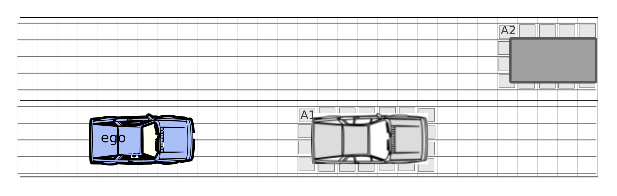
\includegraphics[width=0.4\textwidth]{ego+artifacts.eps}
	\caption{Ego's perceptions}\label{fig:artifacts}
\end{figure}
Let the learning components have determined (based on the sensor measurements) that $A_1$ is some vehicle and that it is not moving. 
Further the learner L(vehicle) classifies $A_2$  with high confidence as a vehicle. Let at time $t$ no other classifier notifies to recognize the artifact --no resolution of percepts is hence required. Based on its beliefs that $A_2$ is a moving vehicle while $A_1$ is a non-moving obstacle, the ego car applies a general dynamics model in its predictions of possible future evolutions and decides that a circumvention of the obstacle is too dangerous since the oncoming traffic might be too fast. As time goes by and ego comes closer to $A_2$ and $A_1$, the classifier for tractor L(tractor) is confident that  $A_2$ is actually tractor.

Since the previous belief of $A_2$ being a vehicle and the new belief of $A_2$ being a tractor is compatible, the resolution component derives that $A_2$ is believed to be a tractor. The prediction engine computes the possible future based on the belief that $A_1$ is a  non moving vehicle and $A_2$ is a tractor and determines that a circumvention maneuver is safe. Since the ego vehicle wants to avoid harsh braking, the maneuver selection determines a maneuver plan to circumvent $A_1$.

This example illustrates that classifications of different detail are relevant for taking the decision on the right maneuver. While it is sufficient to classify $A_1$ as a non-moving obstacle, the decision is highly sensitive to a more precise classification of $A_2$ the oncoming vehicle.


In our scenario, ego prioritizes collision-avoidance over driving fast, it hence is interested in having a classification with a high specificity, i.e., ego wants to know that there is no tractor. Moreover ego can only base its decision on such a classification if the classifier is sufficiently good. We assume that for a safety critical decision, a very high specificity on the test data set is required.
In order to allow optimal decision for achieving the less prioritized goal of driving fast, high sensitivity of the classifier is needed, i.e., ego wants to know whether there is a tractor, because then ego can overtake. Since we here the goal is of less priority, we require that the sensitivity may be less than the specificity. 

Since the currently active list of goals change over time (driving fast to an appoint, but after the appoint driving more relaxed), the requirements on the classifiers change over time as well.  






\section{Proving Safe Perception}\label{sec:proofrule}
Willem and Martin\\
4,5 pages	concluded at page 13\\

\section{Conclusion}

Werner
0,5 page	concluded at page 15

\bibliographystyle{splncs04}
\bibliography{references.bib}

\end{document}
